\documentclass[11pt]{beamer}
\usetheme{Madrid}

\usepackage[spanish]{babel}
\usepackage{amsmath}
\usepackage{amsfonts}
\usepackage{amssymb}
\usepackage{graphicx}
\usepackage{enumerate}
\usepackage{fancyhdr}
\usepackage{fancybox}
\usepackage{lastpage}
\usepackage{color}
\usepackage{amsbsy}
\usepackage{amsthm}
\usepackage{listings}


\usepackage{multirow}
\usepackage{subfig}
\usepackage{textcomp}
\usepackage{makeidx}%glosario de términos

\numberwithin{equation}{section}
\theoremstyle{definition}
\newtheorem{defi}{Definición}[section]

\theoremstyle{definition}
\newtheorem{propo}{Proposición}[section]

\theoremstyle{definition}
\newtheorem{coro}{Corolario}[section]

\theoremstyle{definition}
\newtheorem{teorema}{Teorema}[section]
\setlength{\textwidth}{5in}

\usepackage{srcltx}%permite la busqueda inversa, si no viene por defecto en la version de LaTeX usada.

% lo siguiente solo usarlo cuando compilo directamente en pdflatex
% si lo uso compilando en latex el {\'\i}ndice no lo hace bien
\usepackage{hyperref}

\hypersetup{colorlinks=true, linkcolor=black, urlcolor=black, citecolor=black}
\hypersetup{bookmarksopen=false, bookmarksnumbered=true} \hypersetup{pdfstartview=FitH}

\author{Pedro Ángel Fraile Manzano}
\title{Revisión de métodos multivariantes supervisados y no supervisados}
\AtBeginSection[]
{
  \begin{frame}<beamer>{Contenidos}
    \tableofcontents[currentsection,currentsubsection]
  \end{frame}
}

\AtBeginSubsection[]
{
  \begin{frame}<beamer>{Contenidos}
    \tableofcontents[currentsection,currentsubsection]
  \end{frame}
}
\author{Pedro Ángel Fraile Manzano}
%\title{}
%\setbeamercovered{transparent} 
%\setbeamertemplate{navigation symbols}{} 
%\logo{} 
%\institute{} 
%\date{} 
%\subject{} 
\begin{document}

\begin{frame}
\titlepage
\end{frame}

\begin{frame}
\tableofcontents
\end{frame}

\input{Documentos Extra/Introducción.tex}

\section{Métodos supervisados}
\begin{frame}{Métodos supervisados}
\begin{columns}
\begin{column}{0.9\textwidth}
\begin{defi}
Son aquellos que buscan inferir una relación estocástica entre dos grupos de variables, predictoras a partir de un conjunto de datos procedentes de observaciones simultáneas de ambos conjuntos. 
\end{defi}

Si se estudian varias variables de manera simultánea, se dividen en los siguientes tipos:\pause
\begin{itemize}
\item Variables predictoras, son las variables independientes, se denotarán por el vector aleatorio $\mathbf{x}=[X_1,\ldots, X_p]$ \pause
\item Variables respuesta, son las variables dependientes, se denotarán como el vector aleatorio $\mathbf{y}=[Y_1,\ldots, Y_K]$ y como $Y$ cuando $K=1$.
\end{itemize}
\end{column}
\end{columns}
\end{frame}

\begin{frame}{Métodos supervisados}
\begin{columns}
\begin{column}{0.9\textwidth}
Se trabajará con muestras aleatorias simples de $N$ observaciones de las $K+p$ variables, obteniéndose las siguientes matrices:
\begin{defi}
Se llama matriz de datos $\mathbf{X}$ a la matriz de tamaño $N\times p$ cuyas filas $\mathbf{x}_i,\enspace i=1,\ldots,N$ representan una observación de las $p$ variables predictoras.
\end{defi}
\begin{defi}
Se llama matriz de respuestas $\mathbf{Y}$ a la matriz de tamaño $N\times K$ cuyas filas $\mathbf{y}_i,\enspace i=1,\ldots,N$ representan una observación de las $K$ variables respuesta.
\end{defi}
\end{column}
\end{columns}
\end{frame}

\begin{frame}{Métodos supervisados}
\begin{columns}
\begin{column}{0.9\textwidth}
Por tanto, se recogen $N$ observaciones $(\mathbf{x}_i,\mathbf{y}_i)$ obteniéndose un vector de longitud $K+p$.

Los métodos supervisados buscan estimar una relación estocástica que se llamará predictor que conocido el valor de las variables predictoras $\mathbf{x}_0$, se pueda hacer una predicción del valor de las variables respuesta $\mathbf{y}_0$, que se denota por $\mathbf{\hat{y}}_0$.
\end{column}
\end{columns}
\end{frame}

\subsection{Métodos lineales para regresión}
\begin{frame}{Métodos supervisados}
\begin{columns}
\begin{column}{0.9\textwidth}
El objetivo de la regresión lineal es estudiar como un conjunto de variables respuesta están relacionadas con una combinación lineal de las variables predictoras. 
\end{column}
\end{columns}
\end{frame}

\begin{frame}{Métodos supervisados}
\begin{columns}
\begin{column}{0.9\textwidth}
Tomamos el modelo en el que: 
\begin{equation}
Y=f(\mathbf{x})+\varepsilon
\end{equation}
donde $\varepsilon$ cumple:
\begin{itemize}
\item $\mathbb{E}(\varepsilon)=0$
\item $Var(\varepsilon)=\sigma^2$
\end{itemize}
A mayores se puede asumir que $\varepsilon\sim N(0,\sigma^2)$
\end{column}
\end{columns}
\end{frame}

\begin{frame}{Métodos supervisados}
\begin{columns}
\begin{column}{0.9\textwidth}
En la regresión lineal se asume que $f$ es de la siguiente manera:
\begin{equation}
f(\mathbf{x})=\beta_0+\sum_{j=1}^p \beta_j X_j
\end{equation}
\begin{itemize}
\item $\beta=[\beta_0,\beta_1,\ldots,\beta_p]^T$ es el vector con los parámetros de regresión.
\item Añadiendo a $\mathbf{x}$ la variable $X_0=1$ se puede expresar f: 
\end{itemize}

\begin{equation}
f(\mathbf{x})=\mathbf{x}\beta
\end{equation}

Tomando $N$ observaciones, se puede obtener el vector $\mathbf{\hat{y}}$:
\begin{equation}\label{eq: predicción}
\mathbf{\hat{y}}=\mathbf{X}\beta
\end{equation}

\end{column}
\end{columns}
\end{frame}


\begin{frame}{Métodos supervisados}
\begin{columns}
\begin{column}{0.9\textwidth}
Se pueden estimar los parámetros de regresión mediante el método de los mínimos cuadrados:
\begin{equation}
\hat{\beta}=(\mathbf{X}^T\mathbf{X})^{-1}\mathbf{X}^T \mathbf{y}
\end{equation}

Sustituyendo en la ecuación \ref{eq: predicción}
\begin{equation}
\mathbf{\hat{y}}= \mathbf{X}(\mathbf{X}^T\mathbf{X})^{-1}\mathbf{X}^T \mathbf{y}
\end{equation}

\end{column}
\end{columns}
\end{frame}




\begin{frame}{Métodos supervisados}
\begin{columns}
\begin{column}{0.9\textwidth}

Supóngase lo siguiente: 
\begin{itemize}
\item $\mathbf{x}\sim N(\mu,\Sigma)$ del que obtenemos la matriz de datos $\mathbf{X}$ de tamaño $N\times p$. 
\item $\mathbf{y}=\mathbf{X}\beta+\varepsilon$ donde $\varepsilon\sim N(0,\sigma^2\mathbf{I}_N)$.
\end{itemize}
\end{column}
\end{columns}
\end{frame}



\begin{frame}{Métodos supervisados}
\begin{columns}
\begin{column}{0.9\textwidth}
Se cumplen las siguientes propiedades: 
\begin{itemize}
\item El vector $\mathbf{y}\sim N(\mathbf{X}\beta,\sigma^2\mathbf{I}_N)$
\item El vector $\hat{\beta}$ es un estimador insesgado.
\item La varianza de $Var(\hat{\beta})=\sigma^2(\mathbf{X}^T\mathbf{X})^{-1}$.
\item El estimador $\displaystyle\hat{\sigma}^2=\dfrac{1}{N-p-1}\sum_{i=1}^N(y_i-\hat{y}_i)^2$ es un estimador insesgado de $\sigma^2$ y además $\displaystyle\hat{\sigma}^2\sim \dfrac{\sigma^2}{N-p-1}\chi_{N-p-1}^2$
\end{itemize}

\end{column}
\end{columns}
\end{frame}

\begin{frame}{Métodos supervisados}
\begin{columns}
\begin{column}{0.9\textwidth}
Se puede definir un estadígrafo de contraste para comprobar si un conjunto de variables es estadísticamente significativo en el modelo. 
\begin{equation}\label{eq: Estimador F}
F=\dfrac{\dfrac{(RSS_0-RSS_1)}{p_1-p_0}}{\dfrac{RSS_1}{N-p_1-1}}\sim F_{(p_1,p_0),(N-p_1-1)}
\end{equation}
\end{column}
\end{columns}
\end{frame}


\begin{frame}{Métodos supervisados}
\begin{columns}
\begin{column}{0.9\textwidth}
En el caso de que tengamos $K$ variables respuesta $Y_1,\ldots, Y_K$ entonces el modelo es:
\begin{equation}
Y_k=\beta_{0k}+\sum_{j=1}^p X_j\beta_{jk}+\varepsilon_k = f_k(\textbf{x})+\varepsilon_k, \quad k=1,\ldots K
\end{equation}
donde $\varepsilon_k \sim N(0,\sigma_k^2)\enspace\forall k=1,\ldots,K$ que pueden o no estar correlacionados. Al tomar $N$ observaciones se puede expresar de manera matricial
\begin{equation}
\mathbf{Y=XB+E}
\end{equation}
donde $\mathbf{E}$ es la matriz $N\times K$ de errores cometidos en cada una de las observaciones.
\end{column}
\end{columns}
\end{frame}

\begin{frame}{Métodos supervisados}
\begin{columns}
\begin{column}{0.9\textwidth}
El método de los mínimos cuadrados, cambia en el caso de que los errores tengan matriz de covarianzas $\mathbf{\Sigma}$ conocida el $RSS$ se define de la siguiente manera: 
\begin{equation}
RSS(\textbf{B},\mathbf{\Sigma})=\sum_{i=1}^N(\mathbf{y}_i-f(\textbf{x}_i)) \mathbf{\Sigma}^{-1} (\mathbf{y}_i-f(\textbf{x}_i))^T
\end{equation}

donde $d(\mathbf{x}_i,\mathbf{x}_j)=\sqrt{(\mathbf{x}_i-\mathbf{x}_j) \mathbf{\Sigma}^{-1} (\mathbf{x}_i-\mathbf{x}_j)^T}$ es la distancia de Mahalanobis entre dos observaciones. 
\end{column}
\end{columns}
\end{frame}


\begin{frame}{Métodos supervisados}
\begin{columns}
\begin{column}{0.9\textwidth}
Se puede utilizar el estadígrafo $F$ de la ecuación \ref{eq: Estimador F} para seleccionar las variables del modelo. 

También se puede definir lo siguiente: 
\begin{defi} 
Llamamos errores cuadrados acumulados penalizados, \emph{PRSS}, a la suma de los cuadrados de los errores cometidos con el modelo lineal que usa el  vector de parámetros $\beta$, añadiendo un término regulador $\lambda >0$: 
\begin{equation}
PRSS(\beta)=\sum_{i=1}^n(\textbf{y}_i-\textbf{x}_i\beta)^2+\lambda\sum_{j=1}^p\beta_j^2
\end{equation}
\end{defi}
Esto permite dar una forma de regular los tamaños de los parámetros $\beta$
\end{column}
\end{columns}
\end{frame}

\subsection{Clasificación}
\begin{frame}{Métodos supervisados}
\begin{columns}
\begin{column}{0.9\textwidth}
La clasificación es el caso donde la variable respuesta es cualitativa. 
Hay dos tareas a realizar:
\begin{itemize}
 \item Discriminación: Estudiar las características que diferencian a cada una de las poblaciones. 
 \item Clasificación: Asignar nuevas observaciones a una de las poblaciones 
\end{itemize}
\end{column}
\end{columns}
\end{frame}


\begin{frame}{Métodos supervisados}
\begin{columns}
\begin{column}{0.9\textwidth}
Si tenemos dos poblaciones $\pi_1, \pi_2$ de las cuales se conocen las funciones de probabilidad de cada una de ellas $f_1,f_2$ , entonces si se conoce la probabilidad de de clasificación de clasificar en la población incorrecta, $P(1|2), P(2|1)$, entonces: 
\begin{equation}
\begin{split}
P(i|\textbf{x}_0)&=\dfrac{P(\textbf{x}_0|i)P(i)}{P(1)P(\textbf{x}_0|1)+P(2)P(\textbf{x}_0|2)}\\&=\dfrac{f_i(\mathbf{x}_0)P(i)}{P(1)f_1(\mathbf{x}_0)+P(2)f_2(\mathbf{x}_0)}
\end{split}
\end{equation}
donde $i=1,2$
\end{column}
\end{columns}
\end{frame}

\begin{frame}{Métodos supervisados}
\begin{columns}
\begin{column}{0.9\textwidth}
Se utilizará el concepto de función discriminante: 
\begin{defi}
Se llama función discriminante, $f_{d}$ aquella que:
\begin{equation}
f_{d}:\mathbf{\Omega}\longrightarrow \mathbb{R},
\end{equation}
donde $\mathbf{\Omega}$ es el espacio de observaciones posibles, definida de tal manera que si $f_{d}(\textbf{x}_0)>0\Rightarrow \textbf{x}_0\in \pi_i$ y en caso contrario $\textbf{x}_0\notin \pi_i$. 
\end{defi}
\end{column}
\end{columns}
\end{frame}

\begin{frame}{Métodos supervisados}
\begin{columns}
\begin{column}{0.9\textwidth}
Teniendo esta definición en mente para dos poblaciones y teniendo  en cuenta el coste de clasificación errónea, se obtiene la siguiente función discriminante:

\begin{equation}
f_d(\mathbf{x}_0)=\dfrac{f_1(\textbf{x}_0)P(1)}{c(1|2)}-\dfrac{f_2(\textbf{x}_0)P(2)}{c(2|1)}
\end{equation}

Si se sustituye $f_1,f_2$ por funciones normales se obtiene la función discriminante: 
\begin{equation}
\begin{split}
f_d(\mathbf{x})&=(\textbf{x}-\mu_1)^T \mathbf{\Sigma}^{-1}(\textbf{x}-\mu_1)+log\left(\dfrac{P(1)}{c(1|2)}\right)\\&-(\textbf{x}-\mu_2)^T \mathbf{\Sigma}^{-1} (\textbf{x}-\mu_2)-log\left(\dfrac{P(2)}{c(2|1)}\right)
\end{split}
\end{equation}

\end{column}
\end{columns}
\end{frame}

\begin{frame}{Métodos supervisados}
\begin{columns}
\begin{column}{0.9\textwidth}

El análisis canónico de poblaciones busca identificar las direcciones de mayor diferenciación entre las distintas $L$ poblaciones.
\begin{defi}
\noindent La covarianza intragrupo de un par de variables en la $l$-ésima población:
\begin{equation}
W_l(X_j,X_{j'})=\dfrac{1}{N_l}\sum_{i\in I_l} (x_{ij}-\overline{x}_{jl})(x_{ij'}-\overline{x}_{j'l})
\end{equation}   
\end{defi}
\begin{defi}
La covarianza intergrupos
\begin{equation}
B(X_j,X_{j'})=\sum_{l=1}^L\dfrac{N_l}{N}(\overline{x}_{jl}-\overline{x}_{j})(\overline{x}_{j'l}-\overline{x}_{j'})
\end{equation}   
\end{defi}

\end{column}
\end{columns}
\end{frame}

\begin{frame}{Métodos supervisados}
\begin{columns}
\begin{column}{0.9\textwidth}

Entonces se buscan combinaciones lineales que maximicen la varianza entre grupos respecto la varianza por tanto, se busca maximizar la función
\begin{equation}
f(\mathbf{a})=\dfrac{\mathbf{a}^T\mathbf{Ba}}{\mathbf{a}^T\mathbf{Ta}}
\end{equation}

Tomando la restricción $\mathbf{a}^T\mathbf{T}\mathbf{a}$ y aplicando los multiplicadores de Lagrange, se obtiene que el vector $\mathbf{a}$ es el vector propio con valor propio máximo $\lambda$ de la matriz $\mathbf{T}^{-1}\mathbf{B}$.

\end{column}
\end{columns}
\end{frame}

\subsection{Redes neuronales}
\begin{frame}{Métodos supervisados}
\begin{columns}
\begin{column}{0.9\textwidth}
Una red neuronal artificial es un modelo predictivo basado en el funcionamiento del cerebro humano.\\ 
Cada neurona recibe la información de las neuronas anteriores, las procesa y manda la señal de salida  a las neuronas siguientes. \\

La ventaja es que este tipo de modelos se pueden escalar para tener la complejidad que requieran los datos a costa de perder interpretabilidad, es por ello que normalmente se utilizan con fines únicamente predictivos. 
\end{column}
\end{columns}
\end{frame}

\begin{frame}{Métodos supervisados}
\begin{columns}
\begin{column}{0.9\textwidth}
Conceptos principales: 
\begin{itemize}
\item Pesos sinápticos.
\item Función de activación.
\item Neurona artificial.
\end{itemize}
\begin{figure}[h]
  \centering
  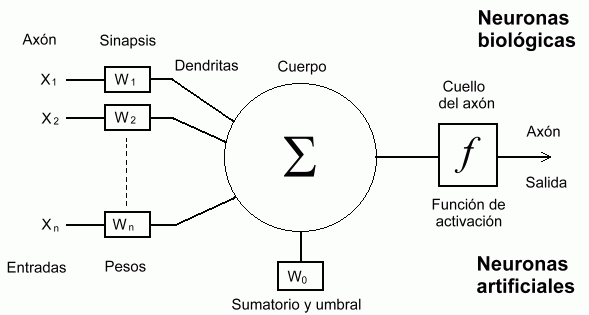
\includegraphics[scale=0.45]{Documentos Extra/Imagenes/neurona.png}
  \caption{Analogía neurona biológica y artificial procedente de \url{https://www.um.es/LEQ/Atmosferas/Ch-VI-3/F63s4p3.htm}}
  \label{fig:neurona}
\end{figure}

\end{column}
\end{columns}
\end{frame}

\begin{frame}{Métodos supervisados}
\begin{columns}
\begin{column}{0.9\textwidth}
Tipos de capas: 
\begin{itemize}
\item Capas de entrada.
\item Capa oculta.
\item Capa de salida.
\end{itemize}

\begin{figure}[h]
  \centering
  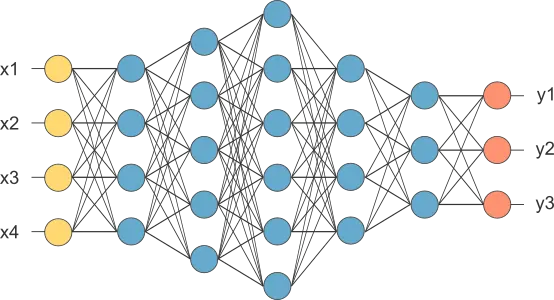
\includegraphics[scale=0.3]{Documentos Extra/Imagenes/red-neuronal-grande.png}
  \caption{Estructura de una red neuronal como un grafo procedente de \url{https://www.neuraldesigner.com/learning/tutorials/neural-network}}
  \label{fig:red neuronal}
\end{figure}
\end{column}
\end{columns}
\end{frame}

\begin{frame}{Métodos supervisados}
\begin{columns}
\begin{column}{0.9\textwidth}
El ajuste de las redes neuronales se realiza con un proceso llamado \emph{backpropagation}. El proceso consiste en los siguientes pasos 
\begin{itemize}
\item Se inicia el modelo con un conjunto de parámetros que puede ser aleatorio o prefijados por el usuario. 
\item Se evalúa la red neuronal con esos parámetros. 
\item Se actualizan los parámetros de acuerdo a algún método de optimización como puede ser el método del gradiente. 
\item Se repiten los dos pasos anteriores hasta que se alcanza algún criterio de parada. 
\end{itemize} 
\end{column}
\end{columns}
\end{frame}



\subsection{Árboles de decisión y bosques aleatorios.}
\begin{frame}{Métodos supervisados}
\begin{columns}
\begin{column}{0.9\textwidth}
\begin{defi}
Los árboles de decisión son conjuntos de reglas discriminantes que fraccionan el espacio de observaciones en regiones donde se modeliza la variable respuesta de manera sencilla. En el proceso de ajuste generan un grafo de tipo árbol con un nodo raíz y los nodos hoja representan cada una de las regiones resultantes. 
\end{defi}
\end{column}
\end{columns}
\end{frame}

\begin{frame}{Métodos supervisados}
\begin{columns}
\begin{column}{0.9\textwidth}
Conceptos importantes:
\begin{itemize}
\item Partición de indices $(j,s)$.
\item Nodo terminal o nodo hoja.
\item Nodo padre y nodo hijo.
\item Profundidad y tamaño del árbol.
\end{itemize}
\begin{center}
\begin{figure}[ht]
  \subfloat[División de $\mathbb{R}^p$]{
   \label{f:división}
    \includegraphics[width=0.25\textwidth]{Documentos Extra/Imagenes/Regiones árboles.png}}
  \subfloat[Diagrama resultante]{
   \label{f:diagrama arbol}
    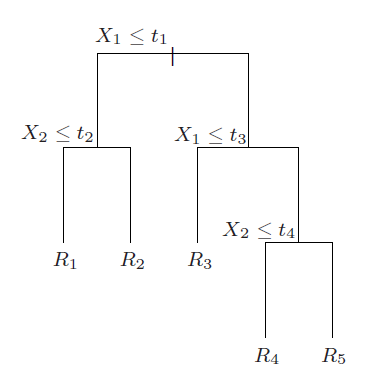
\includegraphics[width=0.25\textwidth]{Documentos Extra/Imagenes/Diagrama de arbol.png}}
 \caption{Representación de la división de $\mathbb{R}^p$ y el diagrama de árbol \\resultante.}
 \label{f:MARC1}
\end{figure}
\end{center}
\end{column}
\end{columns}
\end{frame}
\subsubsection{Árboles de regresión}
\begin{frame}{Métodos supervisados}
\begin{columns}
\begin{column}{0.9\textwidth}
\textbf{Árboles de regresión}

Sea el caso en el que la variable respuesta es cuantitiva y las variables predictoras son cuantitativas o cualitativas.

Tras haber ajustado el árbol hasta tener un tamaño $|T|=M$ resultando en las regiones $R_1,\ldots, R_M$. Entonces el predictor será el siguiente: 
\begin{equation}
\hat{f}(\mathbf{x})=\sum_{m=1}^M \hat{f}_m(\mathbf{x})\cdot \mathbf{1}_m(\mathbf{x})
\end{equation}
donde $\mathbf{1}_m(\mathbf{x})$ es la función característica de la región $R_m,\enspace \forall m=1,\ldots, M$.
\end{column}
\end{columns}
\end{frame}

\begin{frame}{Métodos supervisados}
\begin{columns}
\begin{column}{0.9\textwidth}
\textbf{Árboles de regresión}

Si en cada región queremos que $\hat{f}_m$ sea una constante, $\hat{c}_m$. Utilizando el método de los mínimos cuadrados teniendo en cuenta la restricción de que sea constante se obtiene que: 
\begin{equation}
\hat{c}_m=\dfrac{1}{N_m}\sum_{i/\mathbf{x}_i\in R_m} y_i
\end{equation}
donde $N_m$ es la cantidad de observaciones que hay en la región $R_m \enspace \forall m=1,\ldots M$
\end{column}
\end{columns}
\end{frame}

\begin{frame}{Métodos supervisados}
\begin{columns}
\begin{column}{0.9\textwidth}
\textbf{Árboles de Regresión}

Una partición $(j,s)$ que particione el espacio en las dos regiones $R_{m_1},R_{m_2}$ es elegida si minimiza la siguiente cantidad:
\begin{equation}
\sum_{i/\mathbf{x}_i\in R_{m_1} } (y_i-\hat{c}_{m_1})^2+\sum_{i/\mathbf{x}_i\in R_{m_2} } (y_i-\hat{c}_{m_2})^2
\end{equation}

\end{column}
\end{columns}
\end{frame}


\section{Métodos no supervisados}
\begin{frame}{Métodos no supervisados}
\begin{columns}
\begin{column}{0.9\textwidth}
Los métodos no supervisados son aquellos que buscan analizar la estructura subyacente de los datos. De esta manera no hay una diferenciación de variables, sino que se analizan las relaciones entre las variables. 
\end{column}
\end{columns}
\end{frame}


\subsection{Análisis de componentes principales}
\begin{frame}{Métodos no supervisados}
\begin{columns}
\begin{column}{0.9\textwidth}
Dado un vector aleatorio $\mathbf{x}$ de longitud $p$. Sea $r=rg(\mathbf{X})$. Entonces se definen las componentes principales:
\begin{defi}
Se definen las componentes principales 
\begin{equation}
Z_j=v_{1j}X_1+\ldots v_{pj}X_p=\mathbf{v}_j^T\mathbf{x}^T \quad j=1\ldots r
\end{equation}

\noindent Donde $\textbf{v}_j$ es un vector columna con $p$ escalares y la nueva variable aleatoria $Z_j$ cumple lo siguiente:
\begin{itemize}
\item Si $j=1$ $Var(Z_1)$ es máxima restringido a $\mathbf{v}_1^T \mathbf{v}_1=1$
\item Si $j>1$ debe cumplir:
\begin{itemize}
\item $Cov(Z_j,Z_i)=0\quad \forall i\neq j $
\item $\textbf{v}_j^T \textbf{v}_j=1$
\item $Var(Z_j)$ es máxima. 
\end{itemize}
\end{itemize}
\end{defi}
\end{column}
\end{columns}
\end{frame}


\begin{frame}{Métodos no supervisados}
\begin{columns}
\begin{column}{0.9\textwidth}
\begin{defi}
Dada una matriz $\textbf{X}\in  \mathbb{M}_{N\times p}(\mathbb{R})$ existe la descomposición en valores singulares :
\begin{equation}
\textbf{X}=\textbf{U}\mathbf{D}\textbf{V}^T
\end{equation}
Donde: 
\begin{itemize}
\item \textbf{U} matriz ortogonal y de tamaño $N \times r$
\item $\mathbf{D}$ matriz de tamaño $r \times r$ diagonal, cuyos elementos no nulos son los valores singulares $\sigma_1\geq\ldots\geq \sigma_r\geq 0$, es decir
\begin{equation}
\mathbf{D}=\begin{pmatrix}
\sigma_1 & 0 & \cdots  & \cdots \\
0 & \sigma_2 & 0 & \cdots\\
\vdots & \vdots & \vdots & \vdots\\
\cdots & \cdots & 0 & \sigma_r
\end{pmatrix}
\end{equation}
\item \textbf{V} matriz ortogonal y de tamaño $p \times r$. 
\end{itemize}
\end{defi}
\end{column}
\end{columns}
\end{frame}

\begin{frame}{Métodos no supervisados}
\begin{columns}
\begin{column}{0.9\textwidth}

Las componentes principales se pueden calcular de dos maneras:
\begin{itemize}
\item Descomposición en vectores y valores propios de la matriz de covarianzas. 
\item Descomposición en valores singulares de la matriz de datos

\end{itemize}
\end{column}
\end{columns}
\end{frame}

\begin{frame}{Métodos no supervisados}
\begin{columns}
\begin{column}{0.9\textwidth}

\begin{defi}
Sea $\textbf{A}\in \mathbb{M}_{N\times p}(\mathbb{R})$. Definimos la norma de Frobenius de la matriz \textbf{A} como:
\begin{equation}
||\textbf{A}||_F=(tr(\textbf{A}^T \textbf{A}))^{\frac{1}{2}}=\left(\sum_{i=1}^{N}\sum _{j=1}^{p}a_{ij}^2\right)^{\frac{1}{2}}
\end{equation}
\end{defi}
\begin{propo}
La norma de Frobenius es invariante a transformaciones ortogonales.
\end{propo}

\end{column}
\end{columns}
\end{frame}



\begin{frame}{Métodos no supervisados}
\begin{columns}
\begin{column}{0.9\textwidth}
\begin{defi}
Se llama matriz reducida de orden $m\leq r$ de $\textbf{X}$ y se denota como $\textbf{X}_m$, a la matriz $N\times m $ resultado de:
\begin{equation}
\textbf{X}_m=\textbf{U}_m\mathbf{D}_m\textbf{V}^T_m
\end{equation}
Donde:
\begin{itemize}
\item $\textbf{U}_m$ matriz ortogonal de tamaño $N \times m$, resultado de tomar de \textbf{U} únicamente la matriz las $m$ primeras columnas. 
\item $\mathbf{D}_m$  matriz cuadrada de tamaño $m$ diagonal con los $m$ primeros valores singulares. 
\item $\textbf{V}_m$ matriz ortogonal de tamaño $p \times m$ obtenida al tomar las $m$ primeras columnas de \textbf{V}.
\end{itemize}
\end{defi}
\end{column}
\end{columns}
\end{frame}

\begin{frame}{Métodos no supervisados}
\begin{columns}
\begin{column}{0.9\textwidth}
\begin{teorema}[De Eckart-Young]
Sea \textbf{A} una matriz de coeficientes reales de tamaño $N\times p$ y rango $r$. Entonces se cumple que :
\begin{equation}
||\textbf{A}-\textbf{B}||_F\leq ||\textbf{A}-\textbf{A}_m||_F \quad \forall \textbf{B}/ rg(\textbf{B})=m \leq r
\end{equation} 
\end{teorema}

El número $m$ de componentes principales se puede elegir teniendo en cuenta la siguiente cantidad:
\begin{equation}
t_m=\dfrac{\sum_{j=1}^{m}\lambda_j} {\sum_{j=1}^{r}\lambda_j}
\end{equation}

La proporción de variabilidad acumulada por las $m$ primeras componentes.

\end{column}
\end{columns}
\end{frame}

\subsection{Análisis factorial}
\begin{frame}{Métodos no supervisados}
\begin{columns}
\begin{column}{0.9\textwidth}

El objetivo principal del análisis factorial es estudiar la existencia de estructuras latentes en conjuntos de datos

Esto se traduce buscando si las variables aleatorias pueden ver su variabilidad explicada por un conjunto menor de factores comunes. 

Por tanto, lo que se busca es expresar la variabilidad del conjunto de datos en términos comunes con el resto y una parte específica. 
\end{column}
\end{columns}
\end{frame}

\begin{frame}{Métodos no supervisados}
\begin{columns}
\begin{column}{0.9\textwidth}
Supóngase un vector aleatorio $\mathbf{x}= [X_1, \ldots, X_p]$ de longitud $p$ con una distribución $N(0,\Sigma)$, centrada sin pérdida de generalidad, donde la matriz de covarianzas $\mathbf{\Sigma}$ es simétrica y definido positiva. El modelo factorial se establece:  
\begin{equation}\label{eq Fact}
X_j= \lambda_{1j}F_1+\ldots+\lambda_{mj}F_m+\psi_j U_j\quad j=1\ldots p 
\end{equation}
\noindent Donde:
\begin{itemize}
\item $\lambda_{kj}$ es la saturación de la $j$-ésima variable en el factor común $k$-ésimo. 
\item $F_k$ es el $k$-ésimo factor común
\item $\psi_j$ es la saturación  específica de la variable $X_j$ en el factor único. 
\item $U_j$ es el factor específico para la variable $X_j$.
\end{itemize}
\end{column}
\end{columns}
\end{frame}


\begin{frame}{Métodos no supervisados}
\begin{columns}
\begin{column}{0.9\textwidth}
\noindent El análisis factorial se apoya en las siguientes hipótesis :
\begin{itemize}
\item Los factores comunes $F_k$ son variables aleatorias que siguen una distribución marginal $N(0,1)$. Además se supondrá que $Cov(F_k,F_{k'})=0, k\neq k', \forall k,k'=1,\ldots, m$. Se suponen completamente independientes de los factores específicos. 

\item Los factores específicos $U_j$ son variables aleatorias con una distribución normal $N(0,1)$ no correladas. Se suponen  completamente independientes de los factores comunes. 
\end{itemize} 

\end{column}
\end{columns}
\end{frame}


\begin{frame}{Métodos no supervisados}
\begin{columns}
\begin{column}{0.9\textwidth}
\begin{defi}
Llamaremos matriz de saturaciones de los factores o matriz de saturaciones, $\mathbf{\Lambda}$ de tamaño $p \times m$ a la matriz :
\begin{equation}
\mathbf{\Lambda}=\begin{pmatrix}
\lambda_{11} & \cdots & \lambda_{1 m}\\
\vdots & \ddots & \vdots\\
\lambda_{p1} & \cdots & \lambda_{pm}
\end{pmatrix}
\end{equation}
\end{defi}
\begin{defi}
Se llama comunalidad de la variable $X_j$, a $h_j^2=\sum_{k=1}^m \lambda_{kj}^2 $ .
\end{defi} 
\end{column}
\end{columns}
\end{frame}

\begin{frame}{Métodos no supervisados}
\begin{columns}
\begin{column}{0.9\textwidth}
\begin{defi}
Llamaremos matriz específica a la matriz diagonal $\mathbf{\Psi}$ de tamaño $p\times p$ a aquella que contiene los términos $\psi_j$ donde $j=1,\ldots , p$:
\begin{equation}
\mathbf{\Psi}=\begin{pmatrix}
    \psi_1 & 0 & \dots & 0 \\
    0 & \psi_2 & \dots & 0 \\
    \vdots & \vdots & \ddots & \vdots \\
    0 & 0 & \dots & \psi_p
\end{pmatrix}
\end{equation}
\end{defi}
\begin{defi}
Se llama especificidad o unicidad de la variable $X_j$ a $\psi_j^2, \forall j=1,\ldots, p$.
\end{defi}
\end{column}
\end{columns}
\end{frame}

\begin{frame}{Métodos no supervisados}
\begin{columns}
\begin{column}{0.9\textwidth}
\begin{propo}
La varianza de la variable aleatoria $X_j$, $\sigma_j^2$, se puede descomponer de la siguiente manera:
\begin{equation}
\sigma_j^2 = \sum_{k=1}^{m}\lambda_{kj}^2+\psi_j^2\quad \forall j=1,\ldots,p
\end{equation}
\end{propo}
\begin{propo}
La covarianza de dos variables $Cov(X_j, X_{j'})$, $\sigma_{jj'}$ cumple que 
\begin{equation}
\sigma_{jj'}=\sigma_{j'j}=\sum_{k=1}^{m}\lambda_{kj}\lambda_{kj'}
\end{equation}
\end{propo}
\end{column}
\end{columns}
\end{frame}

\begin{frame}{Métodos no supervisados}
\begin{columns}
\begin{column}{0.9\textwidth}
\begin{teorema}\label{Descomposición Varianza}
La matriz $\mathbf{\Sigma}=\mathbf{\Lambda}\mathbf{\Lambda}^T+\mathbf{\Psi}^2$
\end{teorema}
\end{column}
\end{columns}
\end{frame}

\begin{frame}{Métodos no supervisados}
\begin{columns}
\begin{column}{0.9\textwidth}
Para la estimación de la matriz de satuaciones hay que tener en cuenta la siguiente descomposición:
\begin{equation}
\mathbf{S=\Lambda\Lambda}^T+\mathbf{\Psi}^2
\end{equation}

Por tanto, la matriz de saturaciones $\mathbf{\Lambda}$ se puede estimar haciendo la descomposición en valores y vectores propios de esta matriz. 
\begin{equation}
\mathbf{S-\Psi^2}=\mathbf{\Lambda\Lambda}^T=\mathbf{UDU}^T
\end{equation}

Si $\Psi=0$ se tiene la descomposición en valores y vectores propios de la matriz de covarianzas muestral. 
\end{column}
\end{columns}
\end{frame}

\begin{frame}{Métodos no supervisados}
\begin{columns}
\begin{column}{0.9\textwidth}
Para poder calcular simultáneamente la matriz de saturaciones la matriz específica se plantea el siguiente proceso iterativo. 
\noindent El método se inicia con $\mathbf{\hat{\Psi}}_0=0$ de tal manera que $\mathbf{S}_0^*=\mathbf{S}$. En cada iteración se efectúan las siguientes operaciones: 
\begin{enumerate}
\item Se calcula $\mathbf{S}_i^*=\mathbf{S-\hat{\Psi}}_i^2$.
\item Se calcula la descomposición $\mathbf{\hat{\Lambda}}_i$ como se ha detallado antes obteniendo $\mathbf{U}_i$ y $\mathbf{D}_i$ de tamaños $p\times m $ y $m\times m$. 
\item Se obtiene la nueva estimación de la $\mathbf{\hat{\Psi}}_{i+1}^2=\mathbf{S}-\mathbf{\hat{\Lambda}}_i\mathbf{\hat{\Lambda}}_i^T$
\end{enumerate}

\end{column}
\end{columns}
\end{frame}

\begin{frame}{Métodos no supervisados}
\begin{columns}
\begin{column}{0.9\textwidth}

El modelo está indeterminado por transformaciones ortogonales.
\begin{equation}
\mathbf{x}^T=(\mathbf{\Lambda T}^T)(\mathbf{Tf}^T)+\Psi\mathbf{u}^T
\end{equation}


Para evitar estas indeterminaciones se suelen imponer dos restricciones:
\begin{equation}
\mathbf{\Lambda}^T \mathbf{\Psi}^{-1}\mathbf{\Lambda} \text{ ó } \mathbf{\Lambda}^T \mathbf{\Lambda} \text{ son diagonales con los valores en orden decreciente }
\end{equation}
\end{column}
\end{columns}
\end{frame}

\begin{frame}{Métodos no supervisados}
\begin{columns}
\begin{column}{0.9\textwidth}
\noindent Para interpretar el modelo factorial hay que tener en cuenta los siguientes aspectos:
\begin{itemize}
\item Proporción de varianza común explicada.
\item Especificidad de cada una de las variables.
\item Saturaciones de cada variable en los factores.
\item Significado de los factores
\end{itemize}

\noindent Una vez interpretados los resultados, se puede llegar a los objetivos del análisis factorial, estudiar la estructura latente de los datos en términos de variabilidades comunes. 
\end{column}
\end{columns}
\end{frame}




\subsection{Análisis de cluster}
\begin{frame}{Métodos no supervisados}
\begin{columns}
\begin{column}{0.9\textwidth}
\textbf{Objetivo:} Agrupar en grupos homogéneos o \emph{clusters} las observaciones o mediciones.

\begin{defi}
Diremos que un \emph{cluster} o conglomerado es un subconjunto de las observaciones que son similares entre sí. 
\end{defi}

Se dice que dos observaciones $\mathbf{x}_i,\mathbf{x}_{i'}$ están relacionadas, $\mathcal{R}$, cuando pertenecen al mismo \emph{cluster}.

\begin{defi}
Se llama \textit{clustering} a la partición que provoca la relación $\mathcal{R}$ del espacio de observaciones. 
\end{defi}

\end{column}
\end{columns}
\end{frame}

\begin{frame}{Métodos no supervisados}
\begin{columns}
\begin{column}{0.9\textwidth}
Tipos de algoritmos de \emph{clustering}:
\begin{itemize}
\item \textbf{Particional} una única partición que se va modificando
\item \textbf{Jerárquico} otorga las posibles particiones desde $N$ \emph{cluster} hasta un sólo \emph{cluster}.
\begin{itemize}
\item \textbf{Aglomerativo: } se empiezan con $N$ \emph{clusters} con una observación en cada uno y se van juntando según un criterio establecido. 
\item \textbf{Divisivo} se empiezan con un \emph{cluster} con todas las observaciones  y se va dividiendo según algún criterio establecido. 
\end{itemize}
\end{itemize}
\end{column}
\end{columns}
\end{frame}

\begin{frame}{Métodos no supervisados}
\begin{columns}
\begin{column}{0.9\textwidth}

Dependiendo de cómo se definan las distancias entre los \emph{clusters} se obtendrá un algoritmo u otro:\\
\begin{itemize}
\item El vecino más proximo: $d(C,C')=\min_{\mathbf{x}_i\in C, \mathbf{x}_{i'}\in C'}(\mathbf{x}_i,\mathbf{x}_{i'})$.
\item El vecino más lejano: $d(C,C')=\max_{\mathbf{x}_i\in C, \mathbf{x}_{i'}\in C'}(\mathbf{x}_i,\mathbf{x}_{i'})$.
\item Enlace medio \begin{equation}
d(C,C')=\dfrac{1}{N_C}\dfrac{1}{N_C'}\sum_{\mathbf{x}_i\in C}\sum_{\mathbf{x}_{i'}\in C'} d(\mathbf{x}_i, \mathbf{x}_{i'}).
\end{equation}

\item Ward:
\begin{equation}
d(C,C')=\dfrac{1}{N_C}\dfrac{1}{N_C'}\sum_{\mathbf{x}_i\in C}\sum_{\mathbf{x}_{i'}\in C'} (d(\mathbf{x}_i, \mathbf{x}_{i'}))^2
\end{equation} 
\end{itemize}

\end{column}
\end{columns}
\end{frame}

\begin{frame}{Métodos no supervisados}
\begin{columns}
\begin{column}{0.9\textwidth}

El proceso que siguen los algoritmos jerárquicos aglomerativos es el siguiente:

\begin{itemize}
\item Se inicia con una partición que tiene $N$ \emph{clusters} con una única observación cada uno.
\item Se calcula la matriz de distancias entre los \emph{clusters}. 
\item Se unen los dos clusters que menor distancia tengan entre ellos. De esta manera, se reduce el número de clusters en 1.  
\item Se repiten los dos pasos anteriores hasta tener un único cluster. 
\end{itemize}
\end{column}
\end{columns}
\end{frame}

\begin{frame}{Métodos no supervisados}
\begin{columns}
\begin{column}{0.9\textwidth}
Estos algoritmos tienen la característica que permiten representar sus resultados como un dendograma.

\begin{defi}
Un dendograma es un diagrama de árbol en el que en el eje horizontal se sitúan las observaciones mientras que en el eje vertical se representan las distancias. Cada nodo representa una unión de los clusters. 
\end{defi}

\end{column}
\end{columns}
\end{frame}

\begin{frame}{Métodos no supervisados}
\begin{columns}
\begin{column}{0.9\textwidth}

Los siguientes dendogramas \ref{fig:complete_linkage} \ref{fig:single_linkage}  son resultado de aplicar un algoritmo jerárquico al conjunto \emph{IRIS} de Fisher.
\begin{figure}[h]
 \centering
  \subfloat[Enlace completo]{
   \label{fig:complete_linkage}
    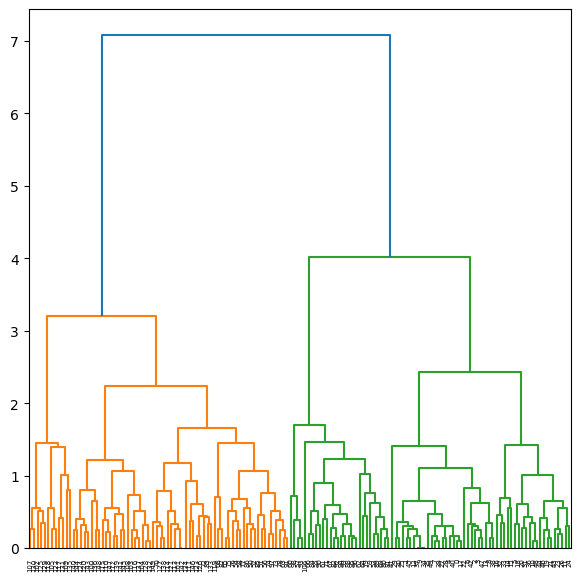
\includegraphics[width=0.35\textwidth]{Documentos Extra/Imagenes/complete_linkage.png}}
  \subfloat[Enlace simple]{
   \label{fig:single_linkage}
    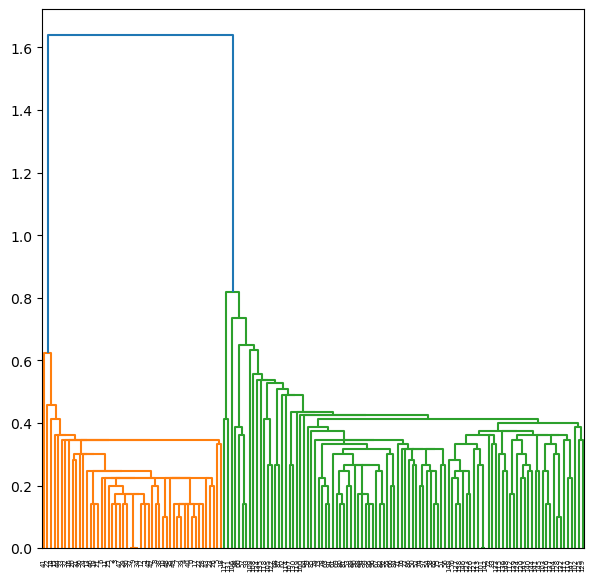
\includegraphics[width=0.35\textwidth]{Documentos Extra/Imagenes/single_linkage.png}}
 \caption{Diagramas obtenidos utilizando la biblioteca de Python Scikit-Learn}
 \label{fig:Dendogramas distintos enlaces }
\end{figure}
\end{column}
\end{columns}
\end{frame}
\begin{frame}{Métodos no supervisados}
\begin{columns}
\begin{column}{0.9\textwidth}

Como se ha dicho, los algoritmos particionales generan un único \emph{clustering} que se va modificando a lo largo de la ejecución del algoritmo.  

Para poder dar el algoritmo más importante de este tipo se necesita del siguiente concepto:

\begin{defi}
Se llama \emph{centroide} de un cluster $C_k,\enspace k=1,\ldots,K$ al vector de tamaño $p$ cuyas componentes son las medias de cada una de las variables de todas las observaciones del \emph{cluster} $C_k$:
\begin{equation}
\overline{x}_{jk}=\dfrac{1}{|C_k|}\sum_{i\in C_k}  x_{ij} \quad \forall j=1,\ldots, p
\end{equation}
\end{defi}
\end{column}
\end{columns}
\end{frame}

\begin{frame}{Métodos no supervisados}
\begin{columns}
\begin{column}{0.9\textwidth}

El algoritmo de $K$-medias se desarrolla de la siguiente manera:

 \begin{enumerate}
\item Se asignan a cada una de las observaciones en cada uno de los $K$ \emph{clusters}. Se calculan los centroides de dichos \emph{clusters}.
\item Se comprueba la distancia euclídea de cada una de las observaciones a los centroides de los \emph{clusters} y se reasignan las observaciones de acuerdo al  más cercano. Tras esto se recalculan los centroides.
\item Se repiten los dos pasos anteriores hasta que las asignaciones no cambien. 
\end{enumerate}
\end{column}
\end{columns}
\end{frame}



\end{document}